\begin{frame}{Example}
    For the waveform $x(t)$,
    \begin{enumerate}
        \item Obtain expression for the exponential Fourier series coefficients $a_k$.
        \item Compute the average power 
        \begin{equation*}
            \frac{1}{T}\int_T |x(t)|^2dt.
        \end{equation*}
        \item Verify Parseval's relation.
    \end{enumerate}
    Given: Sum of the reciprocals of the positive square integers is  $\sum_{k=1}^{\infty}\frac{1}{k^2} = \frac{\pi^2}{6}$.
        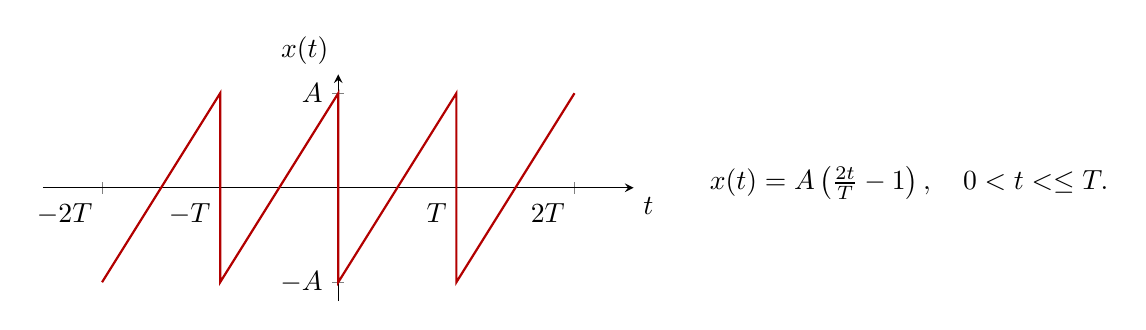
\begin{tikzpicture}[>=latex]
        \begin{axis}[
            x = 1.5cm,
            y = 0.6cm,
            domain=-2:2,
            no markers,
            axis x line=center,
            axis y line=center,
            xlabel style={below right},
            ylabel style={above left},
            xlabel = {$t$},
            ylabel = {$x(t)$},
            ytick={-2, 2},
            yticklabels = {$-A$, $A$},
            xtick={-2,-1, 0, 1, 2},
            xticklabels = {$-2T$, $-T$, 0, $T$, $2T$},
            xticklabel style={below left},
            xmin=-2.5,
            xmax=2.5,
            ymin=-2.4,
            ymax=2.4
            ]
            \addplot[thick, color=red!70!black] coordinates {(-2, -2) (-1, 2) (-1, -2)
            (0,2) (0, -2) (1, 2) (1,-2) (2, 2)};
        \end{axis}
        \pause
        \node at (11,1.5) {$x(t) = A\left(\frac{2t}{T} - 1\right), \quad 0 < t < \leq T.$};
    \end{tikzpicture}
\end{frame}

\begin{frame}
Example: Computing $a_k$
    \begin{columns}
        \begin{column}{0.5\textwidth}
            \begin{align*}
                a_0 &= \frac{1}{T}\int_T x(t)dt\\
                &= \frac{A}{T}\int_0^T \left(\frac{2t}{T} - 1\right)dt\\
                &= \left[\frac{2t^2}{2T}-t\right]_0^T\\
                &= 0
            \end{align*}
            \pause
            \begin{align*}
                a_k &= \frac{1}{T}\int_T x(t)e^{-jk\omega_0 t}dt\\
                    &= \frac{A}{T}\int_0^T \tikzmark{u}\left(\frac{2t}{T} - 1\right) \tikzmark{dv}e^{-jk\omega_0 t}dt\\
                    &=  \frac{A}{T}\left\{ \left[ \left(\frac{2t}{T}-1\right)\frac{e^{-jk\omega_0 t}}{-jk\omega_0}\right]_0^T -  \left[\frac{e^{-jk\omega_0 t}}{-jk\omega_0}\frac{2}{T}\right]_0^T\right\}
            \end{align*}
            \begin{tikzpicture}[
              remember picture,
              overlay,
              expl/.style={draw=orange,fill=orange!30, text centered},
              arrow/.style={red!80!black,ultra thick,->,>=latex}
            ]
            \node<2->[expl,text width=0.8cm]
              (u)
              at ([xshift=4.8ex, yshift=5ex]{pic cs:u})
              {$u$};
            \node<2->[expl, text width=1.2cm]
              (dv)
              at ([xshift=4.8ex, yshift=4ex]{pic cs:dv})
              {$dv$};
            \end{tikzpicture}
        \end{column}
        \begin{column}{0.5\textwidth}
        \pause
            \begin{align*}
                a_k &= \frac{A}{T}\left\{
                 \left[ \left(2-1\right)\frac{e^{-jk\tikzmark{omega0t}\omega_0 T}}{-jk\omega_0} - \frac{(-1)}{-jk\omega_0}\right]\right.\\
                 &-  \left.\frac{2}{-jk\omega_0T}\left[e^{-jk\omega_0T} - 1\right]
                 \right\}\\
                 &= \frac{A}{T}\left\{ \frac{-2}{jk\omega_0} \right\}\\
                 &= \frac{Aj}{\pi k}.
            \end{align*}
            \begin{tikzpicture}[remember picture, overlay]
            \node<3->[draw=orange,fill=orange!30,text width=1.2cm]
              (u)
              at ([xshift=2.4ex, yshift=6ex]{pic cs:omega0t})
              {$\omega_0T = 2\pi$};
            \end{tikzpicture}
            \pause
            \begin{equation*}
                a_k = \begin{cases} 0, & k = 0,\\ \frac{Aj}{\pi k},& k \neq 0.\\
                \end{cases}
            \end{equation*}
        \end{column}
    \end{columns}
\end{frame}


\begin{frame}
Example: Computing the Average Power
    \begin{align*}
        \frac{1}{T}\int_T |x(t)|^2dt &= \frac{A^2}{T}\int_0^T  \left(\frac{2t}{T} - 1\right)^2dt\\
        &=  \frac{A^2}{T}\int_0^T  \left[ \frac{4t^2}{T^2} - 4\frac{t}{T} + 1\right]\\
        &=  \frac{A^2}{T}\int_0^T  \left[ \frac{4t^3}{3T^2} - 4\frac{t^2}{2T} + t\right]\\
        &=  \frac{A^2}{T}\left[ \frac{4}{3T} - 2T + T\right]_0^T\\
        &= \frac{A^2}{3}
    \end{align*}
\end{frame}



\begin{frame}
Example: Verifying Parseval's realtion
    \begin{align*}
        \sum_{k=-\infty}^{\infty}|a_k|^2 &= \sum_{k \neq 0}\left|\frac{Aj}{\pi k} \right|^2\\
        &=  2\frac{A^2}{\pi^2}\sum_{k \neq 1}^{\infty}\frac{1}{ k^2}\\
        &= 2\frac{A^2}{\pi^2}\frac{\pi^2}{6}\\
        &= \frac{A^2}{3}        
    \end{align*}
    \begin{tikzpicture}[
      remember picture,
      overlay,
      expl/.style={draw=orange,fill=orange!30, text centered},
    ]
    \node[expl] at (12,4) {$\sum_{k=1}^{\infty}\frac{1}{k^2} = \frac{\pi^2}{6}$};
    \end{tikzpicture}
\end{frame}


